\subsection{Distribución de Boltzmann}{\label{ap:boltzmann}}

La distribución de Boltzmann se da para todos los sistemas (interactuantes o no) de partículas distinguibles (o clásicas) cuyos potenciales sean independientes de los momentos.
Estos Hamiltoneanos tienen la forma
\[ H(\mathbf{q}_1,..,\mathbf{q}_N,\mathbf{p}_1,..,\mathbf{p}_N) = \sum_{i=1}^N \frac{p_i^2}{2m_i} + U(\mathbf{q}_1,..,\mathbf{q}_N)\]
donde $p_i = |\mathbf{p}_i|$ es el modulo del momento.

Sabiendo que los ensambles son equivalentes en el límite termodinámico, haremos este desarrollo en ensamble canónico por simplicidad.
En este ensamble, la (densidad de) probabilidad de un dado microestado $x=(\mathbf{q}_1,..,\mathbf{q}_N,\mathbf{p}_1,..,\mathbf{p}_N)$ está definida por

\[ P(x) = \frac{e^{-\beta H(\mathbf{q}_1,..,\mathbf{q}_N,\mathbf{p}_1,..,\mathbf{p}_N)}}{\int e^{-\beta H} d^{3N}qd^{3N}p} \]

Aprovechando la forma del Hamiltoneano, la integral del denominador puede factorizarse

\begin{align*}
\int e^{-\beta H} d^{3N}qd^{3N}p &= \int e^{-\beta \left( \sum_i p_i^2/2m_i + U(\mathbf{q}_1,..,\mathbf{q}_N)\right)} d^{3N}qd^{3N}p \\
&= \left(\prod_{i=1}^N\int e^{-\beta\frac{p^2}{2m_i}} d^{3}p\right) \int e^{-\beta U(\mathbf{q}_1,..,\mathbf{q}_N)} d^{3N}q
\end{align*}

Podemos entonces preguntarnos cual es la probabilidad de que una dada partícula $i$ tenga momento $\mathbf{p}_i$.
Esta probabilidad $f_i(\mathbf{p}_i)$ se obtiene integrando sobre todos los posibles estados de las demás partículas y sobre la posición $\mathbf{q}_i$ de la partícula $i$.
Analogamente a la cuenta anterior, vemos que esto arroja

\[ f_i(\mathbf{p}_i) = e^{-\beta\frac{p_i^2}{2m}}\frac{\left(\prod_{j=1, j\neq i}^N\int e^{-\beta\frac{p^2}{2m_j}} d^{3}p\right) \int e^{-\beta U(\mathbf{q}_1,..,\mathbf{q}_N)} d^{3N}q}
{\left(\prod_{j=1}^N\int e^{-\beta\frac{p^2}{2m_j}} d^{3}p\right) \int e^{-\beta U(\mathbf{q}_1,..,\mathbf{q}_N)} d^{3N}q}
= \frac{e^{-\beta\frac{p_i^2}{2m_i}}}{\int e^{-\beta\frac{p^2}{2m_i}} d^3p} \]

Efectuando la integral del denominador, obtenemos finalmente la probabilidad de un dado impulso $\mathbf{p}_i$.
\begin{equation}{\label{eq:dist_MB_imp}}
f_i(\mathbf{p}_i) = \left(\frac{\beta}{2\pi m_i} \right)^{3/2} e^{-\beta\frac{p_i^2}{2m_i}}
\end{equation}
conocida como distribución de Maxwell-Boltzmann.

Dado que esta probabilidad es isótropa, resultaría natural plantearla en función del módulo del impulso para volverla una distribución de una única variable.
Para esto, debemos integrar en todas las posibles direcciones del vector $\mathbf{p}_i$ además de introducir un jacobiano.
Podemos obtener la nueva distribución aprovechando la normalización y realizando el cambio de variables a esféricas
\[1 = \int f_i(\mathbf{p}_i) d^3p = \int_0^\infty\int_0^{4\pi}\left(\frac{\beta}{2\pi m_i} \right)^{3/2} e^{-\beta\frac{p_i^2}{2m_i}} p^2d\Omega dp
= \int_0^\infty 4\pi\left(\frac{\beta}{2\pi m_i} \right)^{3/2} p_i^2 e^{-\beta\frac{p_i^2}{2m_i}} dp_i\]
por lo que la probabilidad de que la $i$-esima partícula tenga un momento con módulo $p$ es
\[ f_i(p) = 4\pi\left(\frac{\beta}{2\pi m_i} \right)^{3/2} p^2 e^{-\beta\frac{p^2}{2m_i}} \]

Sin embargo, si todas las partículas son diferentes (por ejemplo, tienen masas $m_i$ diferentes) esta distribución tiene poco valor estadístico, pues no nos otorga información
del sistema en su totalidad.
Sin embargo, analizar la probabilidad de que la partícula tenga una dada energía cinética $\varepsilon = p^2/2m_i$ permitirá independizarnos de la masa.
Analogamente a lo anterior, planteamos normalización y utilizamos el cambio de variables $2m_i\varepsilon = p^2$ con $d\varepsilon = pdp/m = \sqrt{2m\varepsilon}dp/m$

\[ 1 = \int_0^\infty f_i(p) dp = \int_0^\infty 4\pi\left(\frac{\beta}{2\pi m_i} \right)^{3/2} e^{-\beta\varepsilon} 2m_i\varepsilon\frac{m_i}{\sqrt{2m_i\varepsilon}} d\varepsilon
= \int_0^\infty 2\pi\left(\frac{\beta}{2\pi m_i} \right)^{3/2} e^{-\beta\varepsilon} (2m_i)^{3/2}\sqrt{\varepsilon} d\varepsilon \]

Por lo tanto, la probabilidad de que la $i$-esima partícula tenga una dada energía cinética $\varepsilon$ es identicamente igual para todas las partículas
\begin{equation}
 f(\varepsilon) = \sqrt{\frac{4\beta^3\varepsilon}{\pi}}e^{-\beta\varepsilon}
\end{equation}
y por lo tanto nos permite obtener una propiedad global del sistema.
Si cada partícula tiene probabilidad $f(\varepsilon)d\varepsilon$ de tener energía cinética $\varepsilon$, entonces la cantidad de partículas con esa energía cinética es $Nf(\varepsilon)d\varepsilon$.
Esta es la distribución de energía cinética del sistema.



\subsection{Cálculo de las funciones de Fermi}

En esta sección, hablaremos del método utilizado para computar las $f_\nu(z)$ con especial interés en el caso $\nu=3/2$ que aparece al buscar $\mu(N,V,T)$
y, en menor medida, el caso $\nu=5/2$ asociado a la presión.

Como dijimos, las funciones de Fermi están definidas según su forma integral, pero pueden expresarse como una serie alternada
\begin{equation}{\label{eq:fermi_func_serie}}
 f_\nu(z) \equiv \frac{1}{\Gamma(\nu)}\int_0^\infty \frac{x^{\nu-1}}{z^{-1}e^x+1} dx = \sum_{l\geq 1} (-1)^{l+1}\frac{z^l}{l^\nu}
\end{equation}
cuya convergencia resulta lenta para $z$ de orden 1 o mayor.
Sin embargo, para toda $f_\nu(z)$ existirá algún $z_\nu < 1$ que nos asegure una convergencia veloz de las sumas parciales
\[ f_\nu(z) \approx \sum_{l=1}^{m} (-1)^{l+1}\frac{z^l}{l^\nu}\]
para $z\leq z_\nu < 1$.
Esto se debe a que podemos acortar burdamente el error por
\[ \left|f_\nu(z) - \sum_{l=1}^{m}(-1)^{l+1}\frac{z^l}{l^\nu}\right| \leq \sum_{l=m+1}^\infty z^l = z^{m+1}\sum_{l=0}^\infty z^l = z^{m+1} \frac{1}{1-z} \]
donde usamos $z\leq z_\nu < 1$ para resolver la suma geométrica.

Es de esta cota de donde obtendremos el $z_\nu$ que nos asegure un error relativo tolerable.
Por ejemplo, para $m=20$ y $\nu = 3/2$, podemos aproximar $f_\nu(z)$ para $z\leq z_\nu = 0.65$ con sumas parciales cuyo error relativo está acotado por
\[\frac{|f_\nu(z) - \sum_{l=1}^{m}(-1)^{l+1}\frac{z^l}{l^\nu}|}{f_\nu(z)} \leq 10^{-3} = 0.1\%\]

Este error es suficientemente bajo como para afirmar que el método es preciso.
Sin embargo, para $z = 0.75$, el error relativo ya escala a un $2\%$ y para $z=0.8$ al $10\%$, por lo que resulta necesario mejorar el método.
Una forma de lograr esto sería aumentando el $m$ de las sumas parciales, pero esto conlleva el problema inherente de que los sumandos son estrictamente crecientes en módulo para $z\geq 1$.
Eventualmente, estos valores pueden ser suficientemente grandes como para incurrir en \texttt{overflows} o cancelaciones catastróficas.

\subsubsection{Algoritmo de Wynn}

Dado que la expresión de las $f_\nu(z)$ como serie de potencias resulta problemática para $z\geq 1$, podemos recurrir a otras formas.
Una de estas es la aproximación de Padé por una función racional (cociente de polinomios)
\[ [L/M]_{f_\nu}(z) \equiv \frac{P_L(z)}{Q_M(z)} \approx f_\nu(z) \]
donde $P_L(z)$ y $Q_M(z)$ son polinomios de grado $L$ y $M$, respectivamente.
Estos polinomios no nos interesan dado que utilizaremos el \textit{algoritmo $\epsilon$ de Wynn} para obtener las aproximaciones diagonales $[p/p]_{f_\nu}(z) = \epsilon(0, 2p)$
donde $\epsilon(n,m)$ está definido recursivamente según
\begin{align*}
 &\epsilon(n, -1) = 0 \\
 &\epsilon(n, 0) = \sum_{l=0}^{n} c_lz^l \\
 &\epsilon(n, m+1) = \epsilon(n+1,m-1) + \frac{1}{\epsilon(n+1,m) - \epsilon(n,m)}
\end{align*}
que, para el caso de las $f_\nu(z)$, son $c_0 = 0$ y $c_l=(-1)^{l+1}/l^\nu$ para $l\geq1$.

Para facilitar la visualización, suelen organizarse los $\epsilon$ en una tabla de doble entrada $n$ y $m$ como se muestra en la \textbf{Figura \ref{fig:wynn_esquema}}.
Allí puede verse claramente que $\epsilon$ deben conocerse para computar $\epsilon(n,m)$.
En particular, en la \textbf{Figura \ref{fig:wynn_ejemplo}} puede verse que (dado que $\epsilon(n,-1)=0$) para computar la aproximación $[p/p]$ basta con computar los $\epsilon(n,m)$ con $0\leq n\leq 2p-m$ y $m\leq 2p$.
Esto corresponde a la mitad superior de la antidiagonal, por lo que la cantidad de cómputos es $(2p)^2/2$.

\begin{figure}[H]
	\centering
	\subfigure[Recurrencia entre elementos]{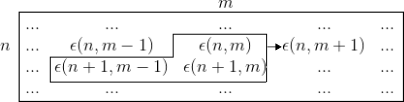
\includegraphics[width=0.26\columnwidth]{apendice/esquema_wynn.png}{\label{fig:wynn_esquema}}}
	\hspace{0.05\columnwidth}
	\subfigure[Ejemplo del cómputo para el caso $p=1$]{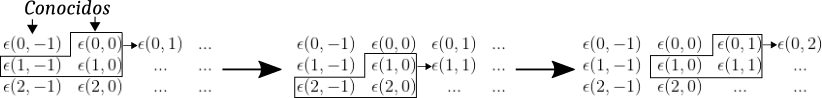
\includegraphics[clip, width=0.68\columnwidth]{apendice/ejemplo_wynn.png}{\label{fig:wynn_ejemplo}}}
	\caption{Arreglo de los coeficientes $\epsilon$ en una tabla para facilitar su cómputo}
	\label{fig:wynn}
\end{figure}

Para una serie de Padé $[p/p]$, el error es $O(z^{2p})$, por lo que tomando $p=10$ podemos obtener un orden similar al de la serie truncada.
Por lo tanto, resultaría razonable utilizar el algoritmo de Wynn para $z\geq z_\nu$, donde (en el caso $\nu=3/2$) empalma con el método de serie truncada con un error
relativo de $\sim10^{-6}$ más que aceptable.

Aunque, en general, las $f_\nu(z)$ no poseen una expresión analítica contra la que podamos comparar la eficacia del algoritmo, el caso particular $\nu=1$ si tiene
expresión analítica: $f_1(z) = \log(z+1)$.
A modo de ejemplo, en la \textbf{Figura \ref{fig:ej_wynn_log}} las aproximaciones a $f_1(z) = \log(z+1)$ mediante el algoritmo de Wynn y sus errores relativos.
Usamos como valor ``exacto'' el arrojado por la función \texttt{log} del paquete \texttt{numpy} de \texttt{Python}.
Puede verse que en el rango $0\leq z\leq 20$, la aproximación con $2p=20$ resulta indistinguible del exacto.

\begin{figure}[H]
	\centering
	\subfigure[Valor absoluto]{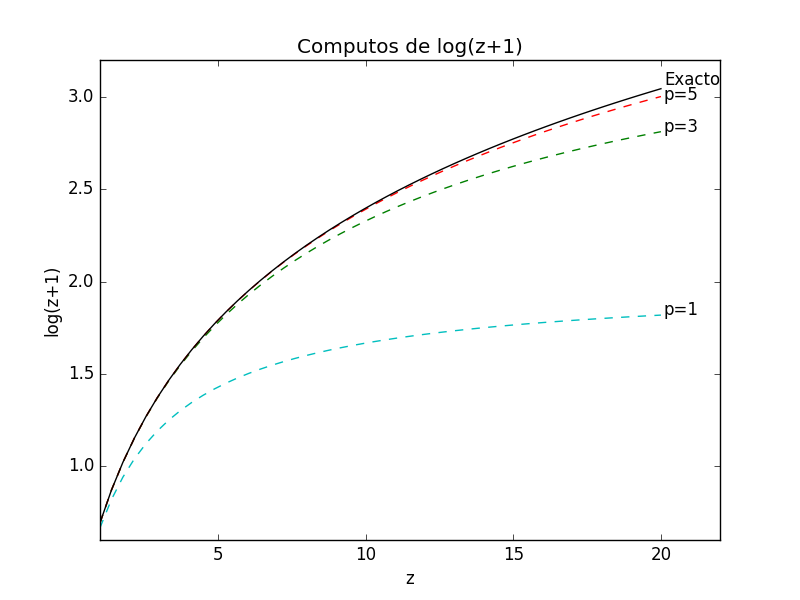
\includegraphics[width=0.4\columnwidth]{apendice/ejemplo_wynn_log.png}}
	\hspace{0.05\columnwidth}
	\subfigure[Error relativo]{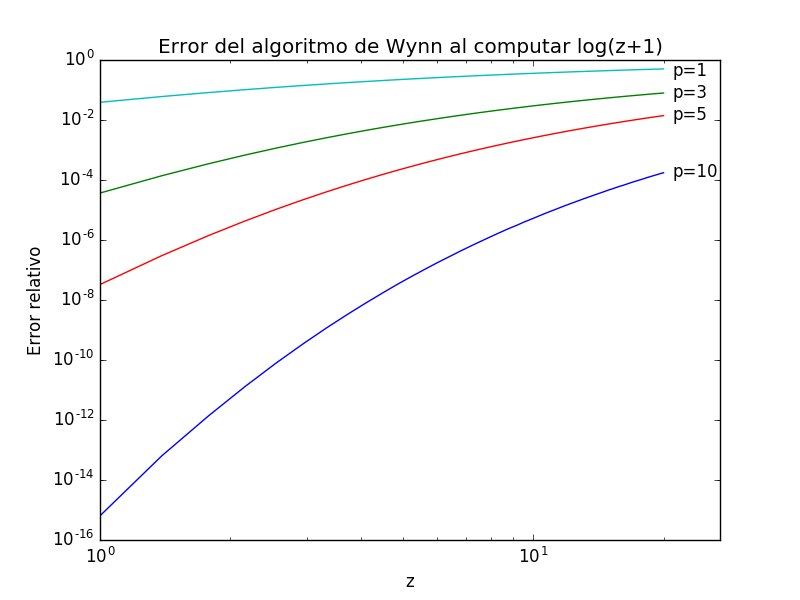
\includegraphics[width=0.4\columnwidth]{apendice/ejemplo_wynn_log_error.png}}
	\caption{Aproximaciones del método de Wynn a la función $f_1(z) = \log(z+1)$, calculada usando el paquete \texttt{numpy} de \texttt{Python}.
	Podemos ver que rapidamente converge a la función para $p=10$, que resulta indistinguible de la exacta.}
	\label{fig:ej_wynn_log}
\end{figure}

Sin embargo, uno podría preguntarse que nos impide utilizar el algoritmo de Wynn en todo el rango de $z$.
Para $z$ pequeño, dado que las sumas parciales de $\epsilon(n,0)$ convergen rapidamente, la resta que aparece en el demonimador de la definición recursiva de
$\epsilon(n, m+1)$ tiende a ser menor al número de máquina, transformándolo en una división por $0$.

Para $z$ suficientemente grande, las sumas parciales de $\epsilon(n,0)$ resultan dominadas por el término $z^n$, con $0\leq n\leq 2p$ y $p\sim 10$.
Por lo tanto, los $\epsilon(n,0)$ se vuelven muy grandes y problemáticos para trabajar para $z\geq 100$.
Para el caso $\nu=3/2$, observamos las primeras inestabilidades para $z\approx 30$.


\subsubsection{Aproximación de Sommerfeld y forma final}

Para $z$ grande, necesitamos otra forma de computar la $f_\nu(z)$.
Surge la pregunta entonces: ¿existe un $z_m$ suficientemente grande para el cual nos baste conocer $f_\nu(z)$ para $z\leq z_m$?
Esta pregunta surge de recordar el objetivo de partida: encontrar el $z$ que cumple $f_\nu(z)=\frac{N\lambda^3}{gV}\equiv \alpha$.
A priori, $\alpha$ no está acotado superiormente, por lo que necesitamos conocer los $z$ para los cuales $f_\nu(z)\to\infty$.
En particular, estamos interesados en que tanto debemos aumentar $z$ para que $f_\nu(z)$ aumente una dada cantidad.

Para esto, utilizamos el conocido lema de Sommerfeld que nos permite aproximar
\begin{equation}{\label{eq:sommerfeld}}
 \int_0^\infty \frac{\Phi(x)}{e^{x-\eta}+1}dx = \int_0^\eta \Phi(x) dx + \frac{\pi^2}{6}\left( \frac{d\Phi}{dx} \right)\Bigg|_{x=\eta} +
 \frac{7\pi^4}{360}\left( \frac{d^3\Phi}{dx^3} \right)\Bigg|_{x=\eta} + ...
\end{equation}

Para el caso de $f_\nu(z)$, podemos usar este lema con $\Phi(x) = x^{\nu-1}/\Gamma(\nu)$ y $z = e^{\eta}$ (o $\eta = \log z$), obteniendo
\begin{equation}{\label{eq:dirac_sommerfeld}}
f_\nu(z) = \frac{1}{\Gamma(\nu)}\left[ \frac{(\log z)^\nu}{\nu} + \frac{\pi^2}{6}(\nu - 1)(\log z)^{\nu-2} + \frac{7\pi^4}{360}(\nu - 1)(\nu - 2)(\nu - 3)(\log z)^{\nu - 4}
+ O((\log z)^{\nu-6})  \right]
\end{equation}

Esto nos dice que para $z$ suficientemente grande, las $f_\nu(z)$ se comportan como potencias del logaritmo de $z$.
Por lo tanto, el crecimiento de $f_\nu(z)$ es considerablemente lento y obtener valores grandes de $f_\nu(z)$ exige valores muchisimo mayores de $z$.
Por ejemplo, utilizar la aproximación de Sommerfeld para resolver $f_{3/2}(z) = 30$ arroja un $z\approx 10^5$.

Para los valores de $z\geq 20$, utilizamos la aproximación \eqref{eq:dirac_sommerfeld} que empalma en $z=20$ con el algoritmo de Wynn con un error relativo de
$\sim10^{-3}$ aceptable (para $\nu=3/2$).

La ventaja de esto es que para $z\geq 20$ tenemos un método explícito y veloz para evaluar $f_{3/2}(z)$, por lo que podemos utilizar algún método para hallar la
raíz de $g(z) = 0 = f_{3/2}(z) - N\lambda^3/gV$ (en nuestro caso, bisecciones).
Por otro lado, para $0\leq z\leq 20$ construimos una Look-Up Table de $\sim 2500$ puntos, interpolando para obtener los valores de $f_\nu(z)$.
En resumen

\[  \left(\nu = \frac{3}{2}\right) \qquad
 \left\{\begin{matrix}
  0 \leq z \leq 20 & \text{Look-Up Table: } \left\{\begin{matrix}
		    0 \leq z \leq 0.65 & \text{Sumas parciales: } f_{3/2}(z) = \sum_{l=1}^{20} (-1)^{l+1} z^l/l^\nu \\
		    0.65 \leq z \leq 20 & \text{Wynn: } \quad f_{3/2}(z) = \epsilon(0,20)
		    \end{matrix}\right. \\
 z\geq 20 & \text{Sommerfeld: } \qquad \qquad f_{3/2}(z) = \frac{4(\log z)^{3/2}}{3\pi^{1/2}}\left[ 1 + \frac{\pi^2}{8}(\log z)^{-2} - \frac{7\pi^4}{384}(\log z)^{-4}  \right]
 \end{matrix} \right.
\]

Para calcular las $f_{5/2}(z)$ asociadas a la presión, debimos aumentar el $z_\nu$ hasta $0.75$ manteniendo el límite inferior de Sommerfeld.
Esta aproximación de la $f_{5/2}(z)$ tiene una calidad similar a la de $f_{3/2}(z)$, como se ve en la \textbf{Figura \ref{fig:f32_f52}}.

\begin{figure}[H]
	\centering
	\subfigure[Función $f_{3/2}(z)$ utilizada para obtener $\mu(N,V,T)$]{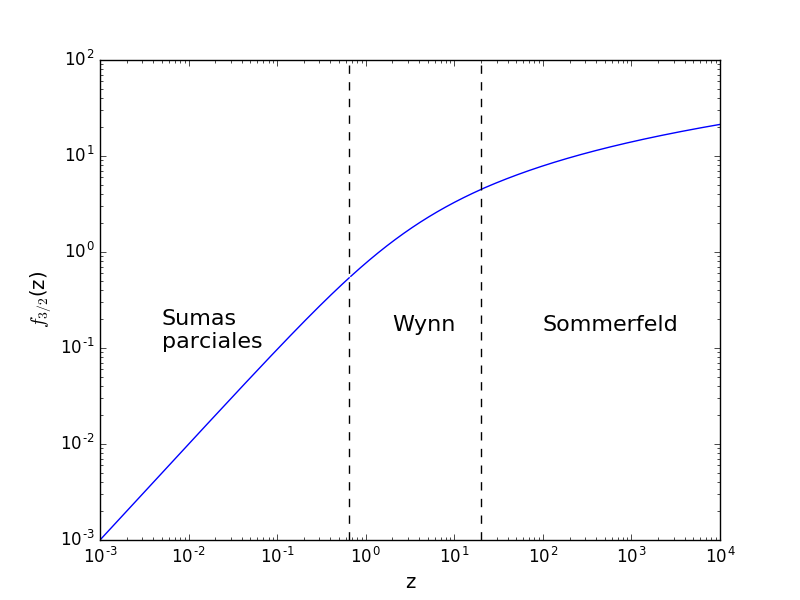
\includegraphics[width=0.4\columnwidth]{apendice/F32.png}}
	\hspace{0.05\columnwidth}
	\subfigure[Función $f_{5/2}(z)$ asociada a la presión del sistema]{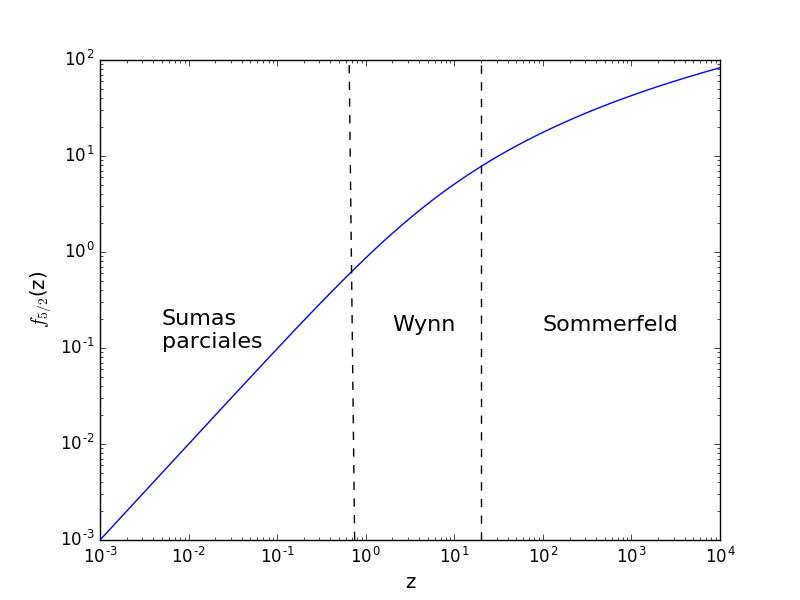
\includegraphics[width=0.4\columnwidth]{apendice/F52.png}}
	\caption{Forma final de las $f_\nu(z)$ utilizando la separación en 3 métodos: sumas parciales, Wynn y Sommerfeld. Puede verse que empalman correctamente.}
	\label{fig:f32_f52}
\end{figure}



\subsection{Teorema del virial}{\label{ap:teo_virial}}

El teorema del virial es un resultado general para sistemas con $q$ y $p$ acotados que surge tanto de la mecánica clásica como de la mecánica estadística.
Nos concentraremos en la versión de mecánica estadística deducida para el ensamble canónico y aprovechando la equivalencia de ensambles en el límite termodinámico.
En particular, analizaremos los valores medios de los observables
\begin{align*}
\left< \dpart{H}{q_i}q_i \right> = \frac{1}{Z}\int \dpart{H}{q_i}q_i e^{-\beta H} d^{3N}qd^{3N}p  &= -\frac{1}{Z\beta}\int q_i \dpart{}{q_i}\left(e^{-\beta H}\right) d^{3N}qd^{3N}p \\
&= -\frac{1}{Z\beta}\int \left[ \cancel{\dpart{}{q_i}\left(e^{-\beta H} q_i\right)} - e^{-\beta H} \right] d^{3N}qd^{3N}p \\
&= \frac{1}{Z\beta}\int  e^{-\beta H} d^{3N}qd^{3N}p = k_B T
\end{align*}
donde hemos usado que el sistema se encuentra acotado en $q$ para cancelar la integral con la derivada.
Podemos hacer un procedimiento análogo para $p_i$ y así obtener
\begin{equation}{\label{eq:teo_virial_T}}
  \left< \dpart{H}{q_i}q_i \right> = k_B T = \left< \dpart{H}{p_i}p_i \right>
\end{equation}

Utilizando las ecuaciones de Hamilton, podemos deducir de \eqref{eq:teo_virial_T} la conocida versión de la mecánica clásica
(donde ahora $\left< \bullet \right>$ corresponde a valor medio temporal)
\begin{equation}{\label{eq:teo_virial_mec}}
  \left< \dot{q}_ip_i \right> + \left< \dot{p}_iq_i \right> = 0 = \frac{d}{dt}\left< q_ip_i \right>
\end{equation}

Dado que ya tenemos una forma de obtener $T$, resulta natural considerar una fórmula para obtener $P$.
Para esto utilizaremos \ref{eq:teo_virial_mec} separando $\dot{p}_i = F_i = F_i^{int}+F_i^{ext}$ y sumando sobre todas las coordenadas del sistema tal que
\[ 0 = \left< \sum_{i=1}^{3N} \dot{q}_ip_i + F_i^{int}q_i \right> + \left< \sum_{i=1}^{3N}F_i^{ext}q_i \right>  \]
donde vemos que el segundo término corresponde a una especie de trabajo de las fuerzas externas que equivale a $-3PV$\textbf{CITA HAILE, APENDICE B}.
Por lo tanto, la presión resulta
\begin{equation}{\label{eq:teo_virial_P}}
P = \frac{1}{3V}\left< \sum_{i=1}^{3N} \dot{q}_ip_i + F_i^{int}q_i \right>
\end{equation}

Para el caso de un potencial no dependiente de momentos, el primer término de la sumatoria se reduce a la energía cinética.
Sin embargo, para un sistema con interacción como la de Pauli agregará un término de \textit{g\"uerzas}.


\subsection{Integradores no simplécticos: Euler y Runge-Kutta}{\label{sec:no_simp}}

En este apéndice, demostraremos que los métodos de Euler y un Runge-Kutta de orden 2 explícitos no son simplécticos.
Comenzaremos con el método de Euler de esquema
\[ y_{n+1} = y_n + h J^{-1} \nabla H(y_n) \]
cuya derivada respecto de $y_n$ resulta inmediatamente
\[ \dpart{y_{n+1}}{y_n} = 1 + hJ^{-1}\nabla^2H (y_n)\]
\begin{align*}
 \left( \dpart{y_{n+1}}{y_n} \right)^T J \left( \dpart{y_{n+1}}{y_n} \right) &= \left(1 + h\nabla^2 H(y_n)(J^{-1})^T\right) J \left(1 + hJ^{-1}\nabla^2 H(y_n)\right) \\
 &= \left(1 - h\nabla^2 H(y_n)J^{-1}\right) J \left(1 + hJ^{-1}\nabla^2 H(y_n)\right) \\
 &= J - \cancel{h\nabla^2 H(y_n)} + \cancel{h\nabla^2 H(y_n)} - h^2\nabla^2 H(y_n)J^{-1}\nabla^2 H(y_n) \neq J
\end{align*}

Por otro lado, el método Runge-Kutta de orden 2 con esquema
\[ y_{n+1} = y_n + h J^{-1} \nabla H\left(y_n + \frac{h}{2} J^{-1} \nabla H(y_n) \right) \equiv y_n + h J^{-1} \nabla H\left(y_{n+1/2} \right) \]
tiene una derivada respecto de $y_n$ más complicada
\begin{align*}
\dpart{y_{n+1}}{y_n} &=  1 - h\left[ 1 - \frac{h}{2} \nabla^2 H(y_n)J^{-1} \right]\nabla^2H\left(y_n + \frac{h}{2} J^{-1} \nabla H(y_n)J^{-1} \right) \\
&\equiv 1 - h\left[ 1 - \frac{h}{2} \nabla^2 H(y_n)J^{-1} \right]\nabla^2H\left(y_{n+1/2} \right) 
\end{align*}
\begin{align*}
 &\left( \dpart{y_{n+1}}{y_n} \right)^T J \left( \dpart{y_{n+1}}{y_n} \right) = \left( 1 - h\left[ 1 - \frac{h}{2} \nabla^2 H(y_n)J^{-1} \right]\nabla^2H\left(y_{n+1/2} \right)J^{-1} \right) J \\
 &\qquad \qquad \qquad \left(1 + hJ^{-1}\nabla^2H\left(y_{n+1/2} \right)\left[ 1 + \frac{h}{2} J^{-1} \nabla^2 H(y_n) \right] \right)\\
 &= J + \frac{h^2}{2} \nabla^2 H(y_n)\nabla^2H(y_{n+1/2}) + \frac{h^2}{2} \nabla^2H(y_{n+1/2})\nabla^2 H(y_n) -\\
 &h^2\left[ 1 - \frac{h}{2} \nabla^2 H(y_n)J^{-1} \right]\nabla^2H(y_{n+1/2}) J^{-1}\nabla^2H(y_{n+1/2})\left[ 1 + \frac{h}{2} J^{-1} \nabla^2 H(y_n) \right] \\
 &= J + \frac{h^2}{2} \left[ \nabla^2 H(y_n)\nabla^2H(y_{n+1/2}) +  \nabla^2H(y_{n+1/2})\nabla^2 H(y_n) - 2\nabla^2H\left(y_{n+1/2} \right) J^{-1}\nabla^2H(y_{n+1/2}) \right] \\
 & + \frac{h^3}{2} \left[ \nabla^2H(y_{n+1/2}) J^{-1}\nabla^2H(y_{n+1/2})J^{-1} \nabla^2 H(y_n) - \nabla^2 H(y_n)J^{-1}\nabla^2H(y_{n+1/2}) J^{-1}\nabla^2H(y_{n+1/2})\right] \\
 & + \frac{h^4}{4} \nabla^2 H(y_n)J^{-1}\nabla^2H(y_{n+1/2}) J^{-1}\nabla^2H(y_{n+1/2})J^{-1}\nabla^2 H(y_n)
\end{align*}

Para anular los ordenes cuadrático y cúbico, se requiere basicamente $\nabla^2H(y_n) = \nabla^2H(y_{n+1/2})$, pero el término cuártico en $h$ es no nulo.
Por lo tanto, este método RK2 no es simpléctico.

\subsection{Implementación de interacción de Pauli}

El objetivo fue generar un método para implementar el cálculo de las fuerzas totales en un sistema de $N_{part}$ partículas para un potencial dado. 
Esta función \texttt{forces} debía ser tan general como fuese posible para así evitar problemas a la hora de cambiar el potencial. 
Implementamos estas funciones en \texttt{C} y, posteriormente, comparamos su velocidad de ejecución para distintas optimizaciones del compilador: \texttt{O0}, \texttt{O1}, \texttt{O2}, \texttt{O3} y \texttt{Ofast}. 

La opción \texttt{O0} es la opción por default en la que no hay optimizaciones mientras que \texttt{O1} es la opción con optimizaciones elementales. 
Por otro lado, la optimización \texttt{O2} realiza todas las optimizaciones que no envuelven \textit{space-speed tradeoff} (mayor uso de memoria en pos de aumentar la velocidad). La opción \texttt{O3}, en cambio, 
si realiza este tipo de optimizaciones como el inlineado de funciones y la vectorización de ciclos. 
Finalmente, la opción \texttt{Ofast} hace todo esto junto optimizaciones que no son \textit{standard-compliant} como \texttt{-ffast-math}; librería con funciones matemáticas implementadas para tener una mayor 
velocidad pero no necesariamente arrojar resultados con la exactitud apropiada. 

Teniendo estas funciones implementadas de la mejor manera, podríamos compilarlas en una librería dinámica y llamarlas desde \texttt{Python}.
De esta manera, podiamos aprovechar la velocidad de cómputo de \texttt{C} junto con la versatilidad de una sesión interactiva de \texttt{Python}.

Con esto en mente, planteamos 9 posibles implementaciones de la función \texttt{forces} combinando distintos rasgos. 
En todos los casos (excepto el primero), \texttt{forces} llamaba otras funciones para ejecutar el cálculo de la fuerza (\texttt{pair\_force}) o energía (\texttt{pair\_energ}) de interacción entre 2 partículas. 
Los rasgos que modificamos fueron: 

\begin{quote}
\begin{description}
\item[Precalculo:] El pre-cálculo o no de parámetros relevantes para la interacción tanto en la energía como en la fuerza de 2 partículas

\item[Auxiliares:] Separar el cálculo auxiliar en 2 funciones distintas \texttt{pair\_force} y \texttt{pair\_energ} o tener una única función \texttt{pair\_energ\_force}

\item[Modulo:] Que la función auxiliar que calcula la fuerza de interacción devuelva el vector completo (con sus 3 componentes) o solo el módulo.
\end{description}
\end{quote}

Comparamos todas estas funciones con una función \texttt{forces1} sin funciones auxiliares que, en principio, sería la más veloz. Así, fue posible evaluar que tanta velocidad de ejecución se perdía en pos de 
la encapsulación del potencial. 

\subsubsection{Estabilización del tiempo de ejecución}

Preliminarmente, buscamos el valor de $N_{part}$ a partir del cual el tiempo de ejecución resultaba $\tau\sim N_{part}^2$ dado que la cantidad de interacciones que \texttt{forces} calculaba es 
$N_{part}(N_{part}-1)/2\sim N_{part}^2$, bajo la hipótesis de que el tiempo de cómputo de la interacción entre 2 partículas es independiente de sus posiciones. 
Para asegurar esto último, evitamos la aplicación de un radio de corte $r_c$ para el potencial (en este caso Morse) que lo anule $\forall r\geq r_c$.

Esto lo hicimos calculando el tiempo que tomaba computar $N_{iter}$ veces las fuerzas de un sistema de $N_{part}$ partículas. 
Los resultados se muestran en la \textbf{Figura \ref{fig:TvsNpart}} y permiten extrapolar que para simulaciones cuya duración sea mayor a $1ms$ o $N_{part}\geq200$, el comportamiento es cuadrático en $N_{part}$.

\begin{figure}[h]
	\centering
	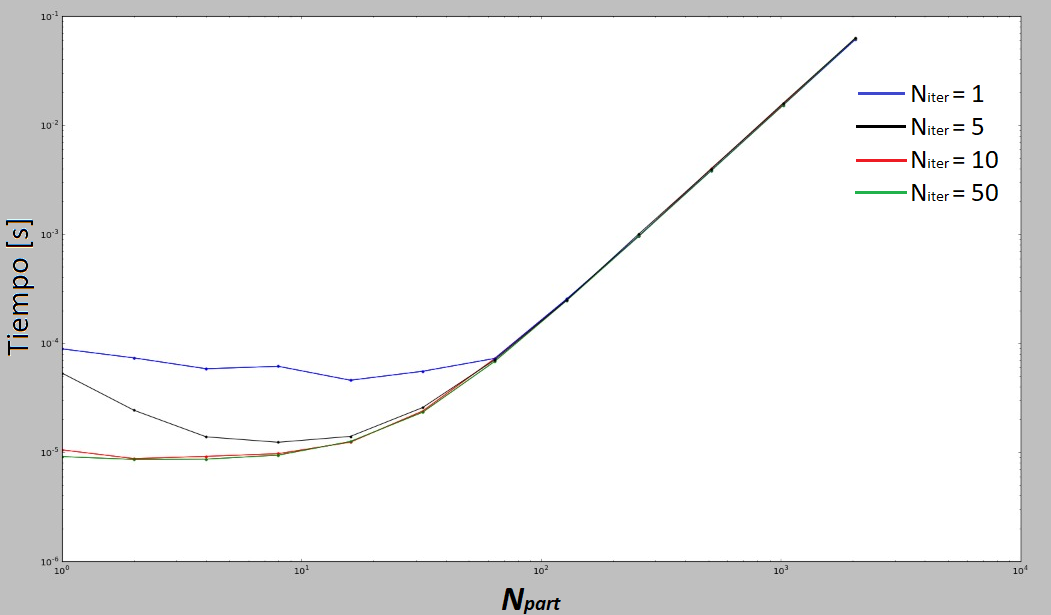
\includegraphics[width=0.65\columnwidth]{apendice/implementacion/Estabilizacion_Npart.png}
	\caption{Tiempo de ejecución de $N_{iter}$ \texttt{forces} para $N_{part}$ partículas. Para $N_{part}>200$ el tiempo ya es polinómico (cuadrático) para todo $N_{iter}$. 
	Esto se condice con simulaciones cuya duración supera $1ms$}
	\label{fig:TvsNpart}
\end{figure}

\subsubsection{Comparación: Potencial de Morse}

El primer potencial que implementamos fue el de Morse
\[ V_{M} (r) = D\left[1-e^{-\alpha (r-r_{eq})}\right]^2\]
dado que su cómputo es muy similar al de Pauli, exigiendo el cálculo de una exponencial.

Realizamos 9 implementaciones del mismo, destacando la implementación 1 por ser la más directa y las funciones 5 y 9 por su mayor portabilidad, además de que devolvian el módulo de fuerza.

\begin{quote}
\begin{description}
\item[1] Sin funciones auxiliares.
\item[5] Dos funciones, con parámetros precalculados, devuelve modulo de fuerza.
\item[9] Dos funciones, sin parámetros precalculados, devuelve modulo de fuerza (encapsula totalmente el potencial).
\end{description}
\end{quote}

\begin{multicols}{3}
\begin{lstlisting}
float forces1(...){
	...
	for(i=0;i<N;i++){
		for(j=i+1;j<N;j++){
			...
			calculo 
			de fuerza
			...
			calculo 
			de energia
			...
		}	
	}
}
\end{lstlisting}
\columnbreak
\begin{lstlisting}
float forces5(...){
	...
	for(i=0;i<N;i++){
		for(j=i+1;j<N;j++){
			...
			precalculo de parametros
			...
			pair_force(params,..)
			pair_energ(params,..)
		}	
		...
	}
	...
}

float pair_force(params,..){
...
}

float pair_energ(params,..){
...
}
\end{lstlisting}

\columnbreak
\begin{lstlisting}
float forces9(...){
	...
	for(i=0;i<N;i++){
		for(j=i+1;j<N;j++){
			pair_force(...)
			pair_energ(...)
		}	
		...
	}
	...
}

float pair_force(..){
	calculo de 
	parametros
	...
}

float pair_energ(..){
	calculo de 
	parametros
	...
}

\end{lstlisting}

\end{multicols}


Esta portabilidad permite usar las 2 funciones auxiliares como \textit{test} directamente desde \texttt{Python} y aprovechan que el vector dirección de la fuerza es independiente del potencial. 
Las demás funciones son:

\begin{quote}
\begin{description}
\item[2 y 3] Única función auxiliar \texttt{pair\_energ\_force} con y sin parámetros precalculados.
\item[4] Como \texttt{forces5} pero devolviendo el vector completo
\item[6] Como \texttt{forces9} pero con algunos parámetros precalculados (no todos).
\item[7 y 8] Versiones de \texttt{forces6} y \texttt{forces9} con una única función auxiliar \texttt{pair\_energ\_force}.
\end{description}
\end{quote}

Compilando con las distintas optimizaciones \texttt{O} corrimos las simulaciones para sistemas con $N_{part}=216$. 
Calculamos el tiempo por par de interacción mediante 
\[ \tau_{par}=\frac{2\tau}{N_{part}(N_{part}-1)} =\frac{\tau}{23220} \]
donde $\tau$ era el tiempo total de duración de la simulación, obtenido mediante estadística sobre $1000$ corridas. 
Los resultados pueden apreciarse en la \textbf{Figura \ref{fig:CompTodas}}.

\begin{figure}[h]
	\centering
	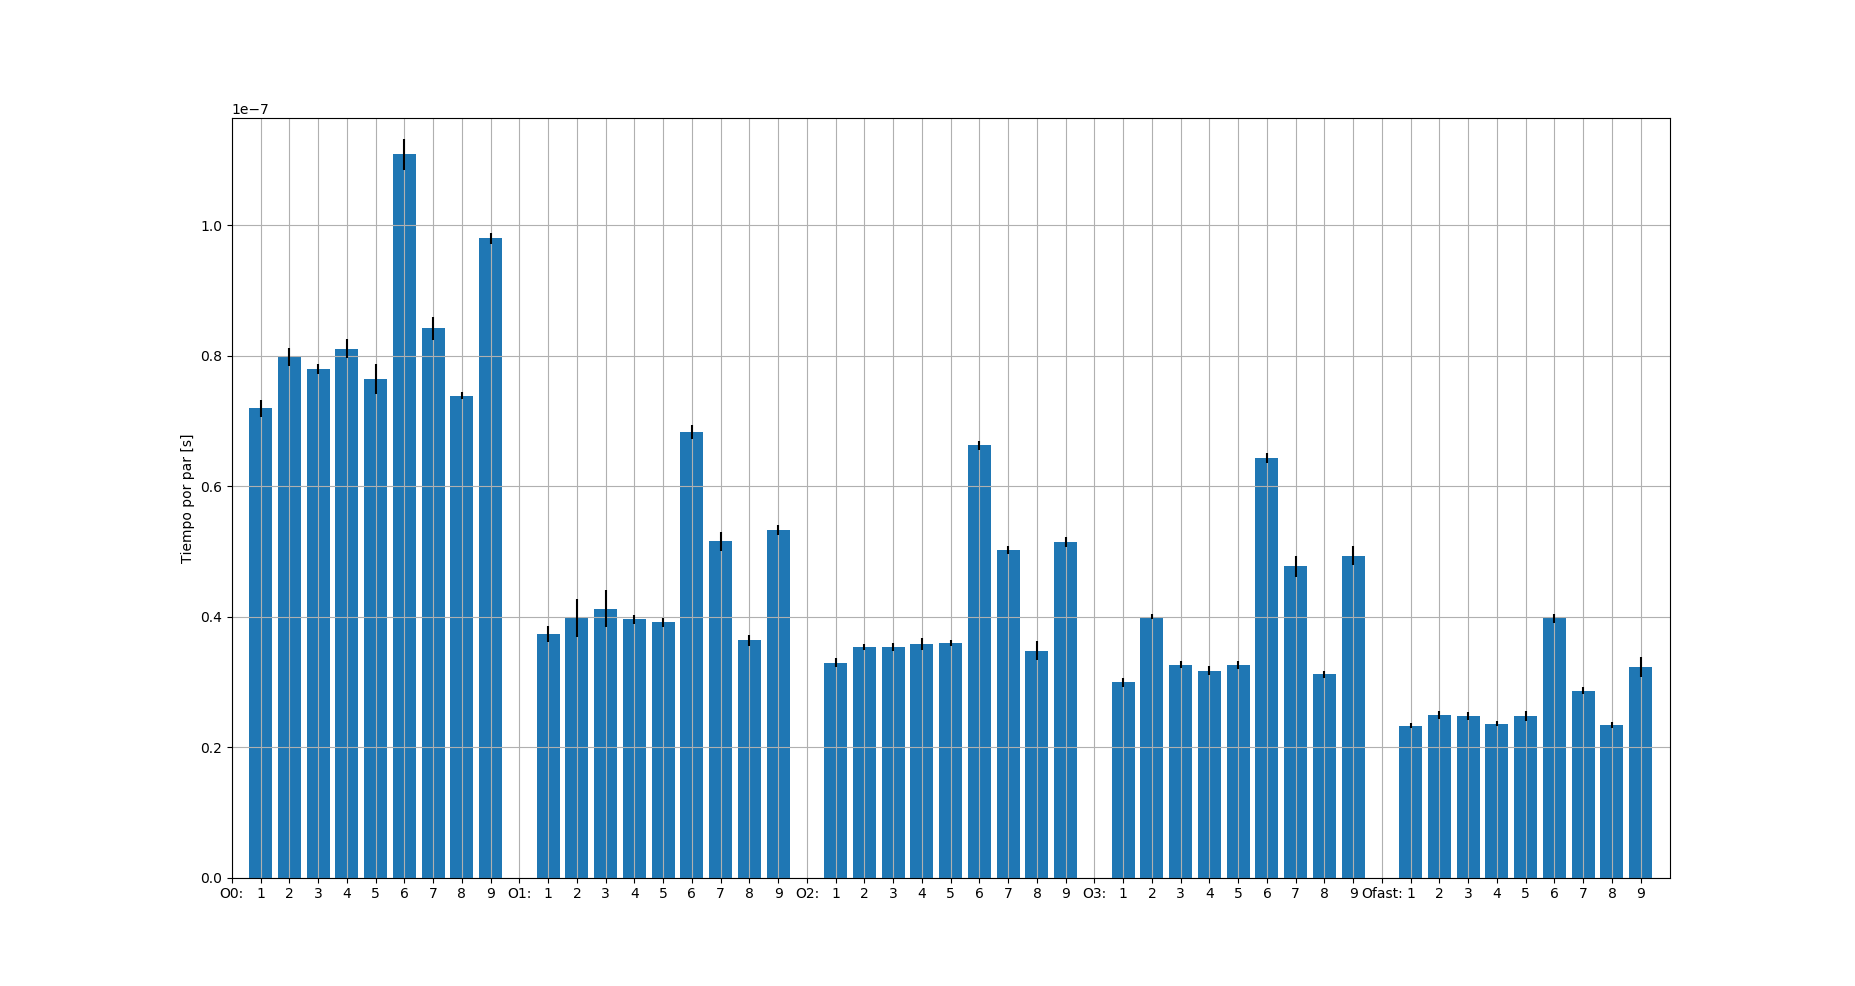
\includegraphics[trim = 40mm 20mm 40mm 20mm, clip, width=\columnwidth]{apendice/implementacion/Comp_tiempos_morse_todos.png}
	\caption{Comparación de tiempos para las distintas implementaciones del potencial de morse. 
	La tendencia decreciente de \texttt{O0} a \texttt{Ofast} es clara, excepto excepciones puntuales de \texttt{O2} a \texttt{O3}.}
	\label{fig:CompTodas}
\end{figure}

En general, puede verse una tendencia decreciente a medida que se pasa de \texttt{O0} a \texttt{Ofast}, lo cual resulta esperable. 
Sin embargo, algunas excepciones notables se dan en el paso de \texttt{O2} a \texttt{O3}.

De mayor interés es notar que el compilador \texttt{Ofast} logra que las implementaciones 2, 3, 4 y 5 tengan diferencias menores al $5\%$ entre si y respecto de la implementación 1, 
volviéndolas virtualmente equivalentes.  
Por tanto, estas 4 implementaciones bien pueden ser reemplazadas unicamente por 5, que resulta más portable como dijimos previamente.

Además, viendo que las implementaciones 6 y 7 tienen tiempos comparables a 9, resulta razonable reemplazarlas por 9. 
En el caso de \texttt{forces9} es importante aclarar que, al no tener ningún parámetro precalculado, la encapsulación del potencial es completa. 
Desde el punto de vista de la ingeniería de software \texttt{forces9} sería la óptima. 

Por lo tanto, aislamos las funciones \texttt{forces1}, \texttt{forces5} y \texttt{forces9} para cuantificar la pérdida de velocidad en pos de la portabilidad (encapsulación del potencial) y 
se volvieron a correr las simulaciones, obteniendo los resultados de la \textbf{Figura \ref{fig:CompEsp}}

\begin{figure}[h]
	\centering
	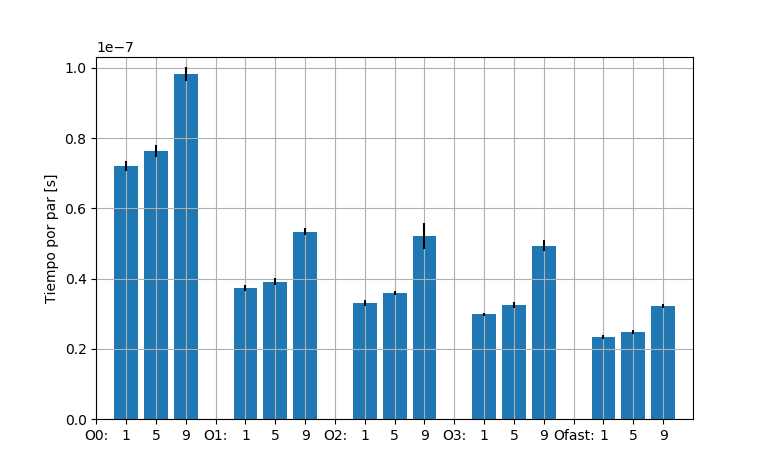
\includegraphics[trim = 10mm 5mm 10mm 5mm, clip, width=0.6\columnwidth]{apendice/implementacion/Comp_tiempos_morse.png}
	\caption{Comparación de las implementaciones de mayor portabilidad (5 y 9) contra la implementación directa 1. 
	Aunque 1 parece equivalente a 5, difiere con 9 en $\sim 40\%$}
	\label{fig:CompEsp}
\end{figure}

Como observamos previamente, la implementación 5 resulta equivalente a la 1 para todos los \texttt{O} (excepto \texttt{O0}). 
Sin embargo, la implementación 9 resulta notoriamente más lenta, con una diferencia relativa respecto a 1 que crece a medida que pasamos de \texttt{O0} a \texttt{Ofast} (donde alcanza un $\sim40\%$). 
Esto último puede deberse a que la separación en 2 funciones obliga a calcular la funcion \texttt{exp} 2  veces, lo cual no ocurre en la implementacion 1 (es directa) ni en la 5 (la exponencial se
pasa como parámetro precalculado). 
Dado que la exponencial no es una función elemental, sus tiempos elevados de calculo pueden causar esta discrepancia.

\subsubsection{Comparación: Potencial de Lennard-Jones}

Con el objetivo de confirmar que la abismal diferencia entre la implementación 9 y la 1 se debe al cálculo de \texttt{exp}, realizamos un análisis similar al anterior para el potencial de Lennard-Jones 
\[ V_{LJ} (r) =  4\varepsilon \left[ \left(\frac{r}{\sigma}\right)^{12} -\left(\frac{r}{\sigma}\right)^{6} \right] \]
que puede calcularse utilizando solamente operaciones algebraicas elementales (multiplicación, suma, resta y división). 
Realizamos las siguientes implementaciones, análogas a 1, 5 y 9 en el caso del potencial de Morse
	
\begin{quote}
\begin{description}
\item[1] Sin funciones auxiliares.
\item[2] Dos funciones, con parámetros precalculados, devuelve modulo de fuerza.
\item[3] Dos funciones, sin parámetros precalculados, devuelve modulo de fuerza (encapsula totalmente el potencial).
\end{description}
\end{quote}

Análogamente, hicimos corridas con cada optimización \texttt{O}, promediando los tiempos con $1000$ corridas. 
Los resultados se encuentran en la \textbf{Figura \ref{fig:CompEsp_LJ}}, donde puede verse el gran salto entre \texttt{O0} y \texttt{O1}, con sus sucesivos saltos de menor orden. 
En particular, entre \texttt{O3} y \texttt{Ofast} no hay ninguna mejora de velocidad. 
Sin embargo, sigue manteniendose la abismal diferencia entre la implementación 9 y la 1 de un $40\%$.

\begin{figure}[h]
	\centering
	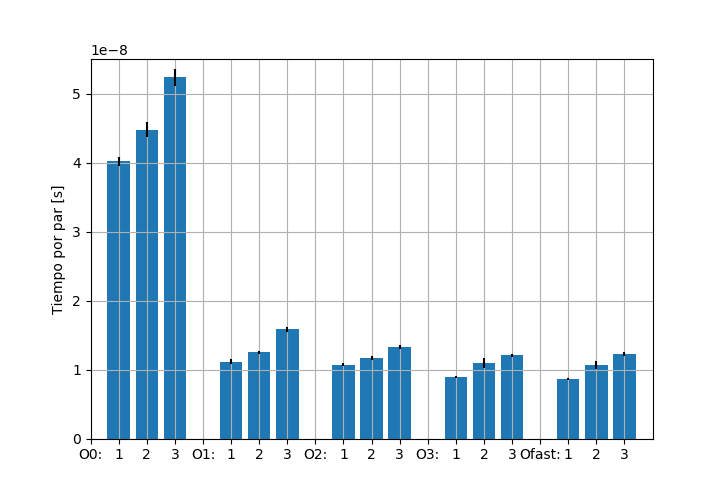
\includegraphics[trim = 10mm 5mm 10mm 5mm, clip, width=0.6\columnwidth]{apendice/implementacion/Comp_tiempos_LJ.png}
	\caption{Comparación de las implementaciones de mayor portabilidad contra la implementación directa 1. 
	A diferencia del caso de Morse, la implementación 2 y 3 resultan notoriamente más lentas que la 1.}
	\label{fig:CompEsp_LJ}
\end{figure}

En particular, comparando las \textbf{Figuras \ref{fig:CompEsp}} y \textbf{\ref{fig:CompEsp_LJ}} puede verse que el cálculo de LJ resulta el doble de rápido que el de Morse. 
Esto permitiría pensar que aproximadamente la mitad del tiempo de cómputo se invierte en calcular \texttt{exp}, hecho que oculta la diferencia real entre la implementación 1 y 5 de Morse, 
que ahora pasa a ser $\sim 20\%$. 

\subsubsection{Inlineado de funciones}

Los resultados previos parecen apuntar al hecho de que los tiempos de simulación se ven afectados por el hecho de que la función \texttt{forces} llame funciones auxiliares \texttt{pair\_force} 
y \texttt{pair\_energ}. 
Este tiempo puede reducirse drásticamente utilizando \textit{function inlining}, que en \texttt{C} se reduce a agregar el sufijo \texttt{inline} delante de la declaración de la función. 
Este inlining fuerza al compilador a copiar la función dentro del cuerpo del código en lugar de llamarla durante su ejecución. 

Dado que las funciones están ahora dentro del cuerpo del código, resulta razonable pensar que los optimizaciones \texttt{O} serán capaces de optimizar la función \texttt{forces} en conjunto 
con \texttt{pair\_force} y \texttt{pair\_energ}. 
Por lo tanto, en el caso del potencial de Lennard-Jones sería factible hacer el cálculo de los parámetros precalculables dentro de \texttt{pair\_force} y \texttt{pair\_energ}, con la esperanza 
de que los optimizaciones lo noten y efectivamente los precalculen fuera de ellas.

Hicimos entonces una versión equivalente a \texttt{forces3} de LJ con estos últimos cambios y se la corrió bajo los mismos parámetros de antes, obteniendo los resultados de la 
\textbf{Figura \ref{fig:CompEsp_LJ_inline}}.

\begin{figure}[h]
	\centering
	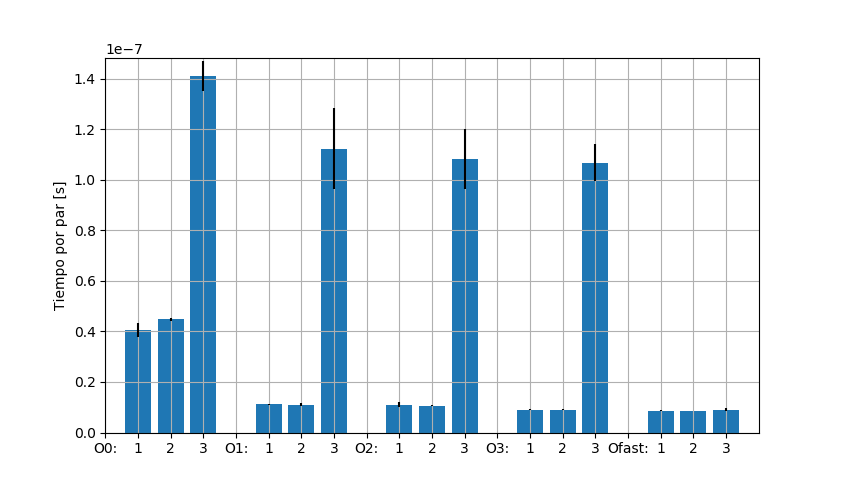
\includegraphics[trim = 10mm 5mm 10mm 5mm, clip, width=0.6\columnwidth]{apendice/implementacion/Comp_tiempos_LJ_inline.png}
	\caption{Comparación de las implementaciones de Lennard-Jones de mayor portabilidad contra la implementación directa 1 utilizando inlining. 
	Solo la optimización \texttt{Ofast} logra volver las implementaciones 1 y 9 comparables; es el único que realiza los precalculos de variables fuera de \texttt{pair\_force} y \texttt{pair\_energ}}
	\label{fig:CompEsp_LJ_inline}
\end{figure}

Los resultados son muy alentadores, dado que las 3 implementaciones resultan indistinguibles dentro del error bajo la optimización \texttt{Ofast}. 
En particular, puede verse como esta modificación resulta terriblemente perjudicial para los los demás optimizaciones, que claramente no realizan el precálculo. 

Finalmente, realizando un trabajo complemente análogo con el potencial de Morse, obtuvimos los resultados de la \textbf{Figura \ref{fig:CompEsp_morse_inline}}. 
Nuevamente, en el caso de \texttt{Ofast} las 3 implementaciones resultan indistinguibles. 
Sin embargo, puede verse como el cálculo de \texttt{exp} nuevamente enmascara las abismales diferencias entre la implementación 1 y 9 para las demás optimizaciones.

\begin{figure}[h]
	\centering
	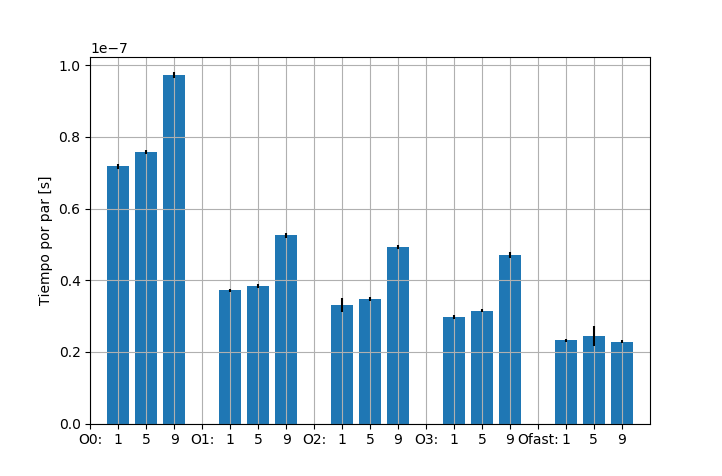
\includegraphics[trim = 10mm 5mm 10mm 5mm, clip, width=0.6\columnwidth]{apendice/implementacion/Comp_tiempos_morse_inline.png}
	\caption{Comparación de las implementaciones de Morse de mayor portabilidad contra la implementación directa 1 utilizando inlining. A diferencia del caso de LJ, la diferencia resulta menos notoria, 
	enmascarada por el cálculo de \texttt{exp}}
	\label{fig:CompEsp_morse_inline}
\end{figure}

Con todo este análisis, resulta inmediato elegir la implementación de \texttt{forces} con dos funciones auxiliares \texttt{pair\_force} y \texttt{pair\_energ} inlineadas sin parametros precalculados, 
que devuelvan el modulo de la fuerza. Esta opción ya era la óptima del punto de vista de ingeniería de software y, gracias al previo análisis, resulta equivalente en términos de velocidad.

Con esto tenemos una encapsulación total del potencial, permitiendo la implementación de un \texttt{forces} como marco general que funciona para cualquier par de funciones auxiliares \texttt{pair\_force} y 
\texttt{pair\_energ}. 
Estas funciones auxiliares son las que introducirán efectivamente el potencial dentro del cálculo; para cambiar el potencial basta cambiar estas funciones auxiliares.

\end{document}
